\documentclass[11pt,a4paper]{article}
\usepackage[spanish,es-noshorthands,es-tabla]{babel}
\usepackage[utf8]{inputenc}
\usepackage[T1]{fontenc}
\usepackage{lmodern}
\usepackage{microtype}
\usepackage[margin=2.2cm]{geometry}
\usepackage{amsmath,amssymb}
\usepackage{graphicx}
\usepackage{booktabs,tabularx}
\usepackage{xcolor}
\usepackage{enumitem}
\usepackage{caption}
\usepackage[section]{placeins}
\usepackage{float}
\usepackage[colorlinks=true,linkcolor=blue!50!black,urlcolor=blue!50!black,citecolor=blue!50!black]{hyperref}
\usepackage{listings}
\lstset{basicstyle=\ttfamily\footnotesize,columns=fullflexible,breaklines=true,frame=single,rulecolor=\color{gray!40}}
\captionsetup{font=small,labelfont=bf}
\setlength{\parskip}{3pt}
\newcommand{\figreg}[2]{\includegraphics[width=0.92\textwidth]{../figuras/#1/#2}}

\title{\textbf{Tarea 1: Descomposición de Fourier Multiescala (MFD)\\ y Envolvente Espectral para diagnóstico de rodamientos}}
\author{Cristóbal Martínez Arochas\\ \small Detección de Anomalías en Sistemas Críticos --- Prof.\ Nibaldo Rodríguez A. --- PUCV}
\date{25 de septiembre de 2026}

\begin{document}
\maketitle

\section{Objetivo}
Diagnosticar el estado de un rodamiento de elementos rodantes con la \textbf{Descomposición de Fourier Multiescala (MFD)} guiada por la curtosis espectral (kurtogram) y la \textbf{envolvente espectral}, usando los datos del Bearing Data Center de la Case Western Reserve University (CWRU). Los objetivos específicos son:
\begin{enumerate}[itemsep=1pt]
\item implementar la MFD;
\item implementar la envolvente espectral;
\item evaluar el rendimiento del diagnóstico.
\end{enumerate}

\section{Datos}
Se usaron los registros CWRU a $F_s=12$~kHz: 60 con falla en el rodamiento del lado de accionamiento (DE, variable \texttt{DE\_time}) y 45 con falla en el lado del ventilador (FE, variable \texttt{FE\_time}). Cubren tamaños de daño de 0{,}007 a 0{,}028~in, cargas de 0 a 3~hp y velocidades de 1720 a 1800~rpm. La carpeta \texttt{data/CWRU} del proyecto también contiene los registros DE a 48~kHz y la línea base normal. El índice \texttt{indice\_cwru.csv} asocia cada archivo con su número CWRU, zona, tamaño y carga.

La frecuencia de giro es $f_r=\mathrm{RPM}/60$ y las frecuencias teóricas de falla son múltiplos cinemáticos de $f_r$ (Tabla~\ref{tab:mult}). Para las fallas de bola se usa $f_d=2\,\mathrm{BSF}$, igual que en el ejemplo de clase (registro 282: $f_d=119{,}5$~Hz), porque la bola golpea ambas pistas por revolución.

\begin{table}[h]
\centering\small
\begin{tabular}{@{}lcccc@{}}
\toprule
Rodamiento & BPFI ($C_i$) & BPFO ($C_o$) & BSF ($C_b$) & FTF\\
\midrule
DE: SKF 6205-2RS JEM & 5{,}4152 & 3{,}5848 & 2{,}3568 & 0{,}3983\\
FE: SKF 6203-2RS JEM & 4{,}9469 & 3{,}0530 & 1{,}9940 & 0{,}3817\\
\bottomrule
\end{tabular}
\caption{Multiplicadores cinemáticos ($f_d=C\cdot f_r$).}
\label{tab:mult}
\end{table}

\section{Método}
\subsection{MFD vía curtosis espectral}
Se implementó exactamente el algoritmo de clase:
\begin{enumerate}[itemsep=1pt]
\item Calcular $X[k]=\mathrm{FFT}\{x[n]\}$ una sola vez.
\item Para $\ell=0,\dots,L$ y $m=0,\dots,2^\ell-1$, construir la máscara simétrica $H_{\ell,m}[k]=1$ si $f^L_{\ell,m}\le|f_k|<f^U_{\ell,m}$, con $\Delta f_\ell=F_s/2^{\ell+1}$, y obtener $x_{\ell,m}[n]=\mathrm{IFFT}\{H_{\ell,m}[k]X[k]\}$.
\item Formar la señal analítica centrada $\tilde z_{\ell,m}$ y calcular la curtosis compleja $K_{\ell,m}=\hat\mu_4/\hat\mu_2^2-2$.
\item Formar el mapa $(f^c,\Delta f,K)$ (kurtogram) y seleccionar $(\ell^\star,m^\star)=\arg\max K_{\ell,m}$.
\item Calcular la envolvente espectral de $x^\star[n]=x_{\ell^\star,m^\star}[n]$.
\end{enumerate}
\textbf{Verificación:} cada nivel reconstruye la señal con un error relativo $\|x-\sum_m x_{\ell,m}\|/\|x\|\approx7\times10^{-16}$.

\textbf{Nivel máximo $L$.} Se usa el mayor $L$ cuyas bandas cumplen $\Delta f_L\ge 2f_d$. La banda filtrada debe contener la modulación de la falla y sus bandas laterales: si $\Delta f<f_d$, la envolvente de la banda ni siquiera puede oscilar a $f_d$. A 12~kHz resulta $L=4$ (bandas de 375~Hz) para casi todos los registros.

\subsection{Envolvente espectral}
Con la definición de clase:
\[
a[n]=\big|x[n]+j\mathcal H\{x[n]\}\big|,\qquad \tilde a[n]=a[n]-\tfrac1N\textstyle\sum_q a[q],\qquad S_{\mathrm{env}}[k]=\big|\mathrm{FFT}\{\tilde a[n]\}\big|^2 .
\]
La transformada de Hilbert se calcula por FFT. Todo el núcleo numérico usa sólo NumPy.

\subsection{Criterio de diagnóstico (objetivo y reproducible)}\label{sec:criterio}
Para clasificar un espectro como \emph{diagnosticable}, \emph{parcialmente diagnosticable} o \emph{no diagnosticable} sin depender de la inspección visual, se usa una prueba de significancia.
\begin{itemize}[itemsep=1pt]
\item Para cada armónica $h f_d$ ($h=1,2,3$) se toma el máximo de $S_{\mathrm{env}}$ en $h f_d\pm2\%$ (tolerancia para el deslizamiento de 1--2\%) y se compara con la media local de $S_{\mathrm{env}}$ en $h f_d\pm0{,}3f_d$, sin contar la ventana del pico.
\item Bajo ruido, los bins de un periodograma son aproximadamente exponenciales. El máximo de $M$ bins supera $k$ veces la media con probabilidad $1-(1-e^{-k})^M$. Se fija esa probabilidad en 1\%, lo que da $k\approx 9{,}1$--$9{,}9$~dB.
\end{itemize}
Con eso:
\begin{itemize}[itemsep=1pt]
\item \textbf{Diagnosticable (D):} la armónica 1 o 2 es significativa \emph{y} es el pico más alto de la envolvente en $[0{,}5f_d,\,3{,}5f_d]$.
\item \textbf{Parcialmente diagnosticable (P):} alguna armónica es significativa, pero no domina el espectro.
\item \textbf{No diagnosticable (N):} ninguna armónica es significativa.
\end{itemize}

%=====================================================================
\section{Resultados}
%=====================================================================
\subsection{Entregable: registro parcialmente diagnosticable (archivo 287)}
\begin{table}[H]\centering\small
\begin{tabular}{@{}ll@{}}\toprule
Bearing & FE (Fan End)\\
Nro. File & 287\\
RPM (Hz) & 1775 rpm ($f_r$ = 29,583 Hz)\\
Load (hp) & 1\\
Damage Size (in) & 0,014\\
Damage Zone & Elemento rodante (ball)\\
Fault Freq. (Hz) & 117,98 ($2\,$BSF)\\
Banda MFD elegida & 3000--4500 Hz ($\ell$=2, m=2, $K$ = 17,9)\\
Diagnóstico señal cruda & Parcialmente diagnosticable\\
Diagnóstico señal filtrada & Parcialmente diagnosticable\\
\bottomrule\end{tabular}
\caption{Ficha del registro 287.}\end{table}

\begin{figure}[H]\centering\figreg{287}{0_kurtogram.png}\caption*{Kurtogram MFD del registro 287 ($L=4$). El máximo está en $\ell=2$, 3000--4500~Hz ($K=17{,}9$).}\end{figure}
\begin{figure}[H]\centering\figreg{287}{1_senal_cruda.png}\\\figreg{287}{2_espectro_senal_cruda.png}\\\figreg{287}{3_envolvente_espectral_cruda.png}\caption*{Registro 287, señal cruda: forma de onda (0{,}5~s), espectro (en sombra, la banda elegida) y envolvente espectral.}\end{figure}
\begin{figure}[H]\centering\figreg{287}{4_senal_filtrada.png}\\\figreg{287}{5_espectro_senal_filtrada.png}\\\figreg{287}{6_envolvente_espectral_filtrada.png}\caption*{Registro 287, señal filtrada en la banda MFD. Hay una joroba ensanchada y significativa en $f_d$ (10{,}9~dB sobre el fondo, con umbral de 9{,}3~dB). $2f_d$ y $3f_d$ se insinúan bajo el umbral, y los picos más altos están en la frecuencia de jaula (FTF $\approx11$~Hz) y su armónica: es la firma típica de una falla de bola con deslizamiento. Como $f_d$ es significativa pero no domina, el registro queda parcialmente diagnosticable, igual que en la categoría P de Smith \& Randall.}\end{figure}

\subsection{Entregable: registro no diagnosticable (archivo 282, ejemplo de clase)}
\begin{table}[H]\centering\small
\begin{tabular}{@{}ll@{}}\toprule
Bearing & FE (Fan End)\\
Nro. File & 282\\
RPM (Hz) & 1798 rpm ($f_r$ = 29,967 Hz)\\
Load (hp) & 0\\
Damage Size (in) & 0,007\\
Damage Zone & Elemento rodante (ball)\\
Fault Freq. (Hz) & 119,51 ($2\,$BSF)\\
Banda MFD elegida & 1500--1875 Hz ($\ell$=4, m=4, $K$ = 161,0)\\
Diagnóstico señal cruda & Parcialmente diagnosticable\\
Diagnóstico señal filtrada & No diagnosticable\\
\bottomrule\end{tabular}
\caption{Ficha del registro 282.}\end{table}

\begin{figure}[H]\centering\figreg{282}{0_kurtogram.png}\caption*{Kurtogram MFD del registro 282. El máximo ($K=161$) está en 1500--1875~Hz: son ráfagas impulsivas muy intensas y aisladas, no periódicas.}\end{figure}
\begin{figure}[H]\centering\figreg{282}{1_senal_cruda.png}\\\figreg{282}{2_espectro_senal_cruda.png}\\\figreg{282}{3_envolvente_espectral_cruda.png}\caption*{Registro 282, señal cruda. En la envolvente de la señal cruda, $2f_d$ y $3f_d$ superan el umbral de significancia (10{,}5 y 10{,}4~dB), pero $f_d$ no lo supera y no son el pico dominante, así que es parcialmente diagnosticable.}\end{figure}
\begin{figure}[H]\centering\figreg{282}{4_senal_filtrada.png}\\\figreg{282}{5_espectro_senal_filtrada.png}\\\figreg{282}{6_envolvente_espectral_filtrada.png}\caption*{Registro 282, señal filtrada. La banda de máxima curtosis concentra impulsos no periódicos: la envolvente queda dominada por ruido de baja frecuencia y $2\,$BSF $=119{,}5$~Hz no es significativa, así que el registro es no diagnosticable. Esto coincide con Smith \& Randall (2015), que clasifican el 282 como N1 para el sensor FE con sus tres métodos.}\end{figure}

\subsection{Evaluación sobre los 105 registros de 12~kHz}
\begin{table}[H]\centering\small
\begin{tabular}{@{}lccc|c@{}}\toprule
 & Diagnosticable & Parcial & No diagn. & Total\\\midrule
Envolvente de la señal cruda & 62 & 40 & 3 & 105\\
Envolvente de la señal filtrada (MFD) & 44 & 33 & 28 & 105\\
\bottomrule\end{tabular}
\caption{Resultado del método en los 105 registros de 12~kHz (criterio de la sección 3.3).}\label{tab:todos}\end{table}
\begin{table}[H]\centering\small
\begin{tabular}{@{}lccc@{}}\toprule
MFD (filtrada) $\backslash$ Smith \& Randall & Y (70) & P (17) & N (18)\\\midrule
Diagnosticable & 43 & 1 & 0\\
Parcialmente diagnosticable & 20 & 7 & 6\\
No diagnosticable & 7 & 9 & 12\\
\bottomrule\end{tabular}
\caption{Contraste con la mejor categoría de Smith \& Randall (2015) para el mismo sensor (Y: diagnosticable, P: parcial, N: no).}\label{tab:sr}\end{table}

\noindent\textbf{Lectura.}
\begin{itemize}[itemsep=2pt]
\item El filtrado MFD entrega un diagnóstico (D o P) en 77 de 105 registros. En 44 registros la señal filtrada es diagnosticable.
\item \textbf{El filtrado no siempre ayuda.} En 19 registros la envolvente cruda ya era diagnosticable y la filtrada dejó de serlo; en 1 ocurrió lo contrario. En 32 registros (31 de ellos DE) el kurtogram elige la banda angosta 5625--6000~Hz, junto a Nyquist, con $K$ que llega a valores del orden de $10^3$. En 20 de esos 32 la envolvente filtrada queda no diagnosticable. En esa banda hay ráfagas impulsivas no relacionadas con la falla. Smith \& Randall describen en CWRU interferencia electromagnética de alta frecuencia y pulsos aparentemente aleatorios, y el kurtogram, que sólo mide impulsividad, los prefiere a la resonancia de la falla.
\item Por sensor, la señal filtrada es D o P en 39 de 60 registros DE y en 38 de 45 registros FE.
\item El contraste con Smith \& Randall (Tabla~\ref{tab:sr}) es coherente: ningún registro que ellos califican como N queda como diagnosticable, y los registros N de la MFD se concentran en sus categorías N y P.
\end{itemize}


\subsection{Comparación visual: método de la tarea vs.\ descenso por sinergia}\label{sec:comp}
El \emph{descenso por sinergia} usa el mismo árbol MFD, pero en lugar de elegir $\arg\max K$ recorre el árbol desde la raíz. En cada nodo pregunta si sus dos hijos están co-modulados, es decir, si los impactos encienden ambas sub-bandas a la vez ($Z\ge3$ en la prueba con surrogados). Si lo están, la banda es ``indivisible'' y se detiene; si no, baja al hijo con mayor curtosis heredada. La teoría y el código están en la carpeta \texttt{02\_Sinergia\_Fraterna} del proyecto. Las figuras de esta sección se generan con \texttt{python comparacion\_descenso.py}.

\subsubsection{Cómo leer las figuras}
Cada figura tiene cinco filas.
\begin{enumerate}[itemsep=1pt]
\item \textbf{Kurtogram} con las dos bandas elegidas (naranjo: kurtogram; azul: descenso; punteado: camino del descenso).
\item \textbf{Envolvente de la banda del kurtogram dividida por su fondo local}, $R(\alpha)=S_{\mathrm{env}}(\alpha)/\bar S(\alpha)$ en dB. $\bar S(\alpha)$ es la media de $S_{\mathrm{env}}$ en $\alpha\pm0{,}3f_d$ sin la ventana de $\pm2\%$: el mismo fondo del criterio de la sección~\ref{sec:criterio}. En esta escala el umbral de significancia es una \emph{línea horizontal} ($\approx9{,}4$~dB) y todo pico que la cruza es una línea discreta real, no ruido. Los picos sobre el umbral se colorean según la familia cinemática a la que pertenecen \emph{por su posición}: armónica de $f_d$, banda lateral ($hf_d\pm kf_r$ en pista interna, $hf_d\pm\mathrm{FTF}$ en bola), armónico de giro $nf_r$, combinación giro--jaula $mf_r\pm n\,\mathrm{FTF}$, u otra. La estrella marca el pico más alto de $S_{\mathrm{env}}$ (en valor absoluto) en $[0{,}5f_d,\,3{,}5f_d]$, la zona sombreada.
\item \textbf{Zoom lineal a $f_d$, $2f_d$ y $3f_d$.} La franja de color es la ventana de búsqueda $\pm2\%$ y la zona gris, los $\pm0{,}3f_d$ usados para el fondo. La línea continua es la media del fondo (1$\times$) y la discontinua, el umbral $k$. El círculo es el pico que eligió el criterio (lleno si es significativo), con su altura en veces el fondo. Los triángulos verdes y morados indican dónde deberían caer los armónicos de giro y las bandas laterales.
\item[4--5.] Lo mismo para la banda del descenso.
\end{enumerate}

\subsubsection{¿Cómo se sabe que un pico es una armónica de \texorpdfstring{$f_d$}{fd}?}\label{sec:armonica}
El registro 107 es un buen ejemplo: en la banda del descenso hay unos 30 picos sobre el umbral. El criterio no intenta explicarlos todos. Hace cuatro comprobaciones, y todas miran lugares fijados \emph{antes} de mirar el espectro:
\begin{enumerate}[itemsep=2pt]
\item \textbf{Posición fijada por la cinemática.} $f_d=5{,}4152\,f_r=157{,}8$~Hz sale de la geometría del rodamiento y de la velocidad; no se busca en el espectro. Sólo se examina $hf_d\pm2\%$, la tolerancia para el deslizamiento de 1--2\% de los elementos rodantes. En el 107 los picos elegidos están en 157{,}4, 314{,}8 y 472{,}1~Hz: razones $1:2{,}000:2{,}999$, con la $f_d$ real 0{,}2\% bajo la teórica. Tres picos en múltiplos exactos de la misma frecuencia forman una \emph{serie armónica}; un pico aislado cerca de $f_d$ no bastaría.
\item \textbf{Altura contra el fondo local, no contra el máximo del espectro.} Bajo ruido, los bins de un periodograma son aproximadamente exponenciales. El máximo de los $M$ bins de la ventana supera $k$ veces la media con probabilidad $1-(1-e^{-k})^M$. Con esa probabilidad en 1\%, $k$ queda entre 8 y 10 veces el fondo (9{,}1--9{,}9~dB, según el ancho de la ventana). En la banda del descenso del 107, las tres armónicas están a 10\,571, 1\,229 y 436 veces el fondo (40{,}2; 30{,}9 y 26{,}4~dB). En la banda del kurtogram, las mismas ventanas llegan sólo a 3{,}7; 5{,}5 y 2{,}9 veces: no se distinguen del ruido.
\item \textbf{Dominancia.} Para ser \emph{diagnosticable}, el pico más alto de $S_{\mathrm{env}}$ en $[0{,}5f_d,\,3{,}5f_d]$ (la estrella) tiene que ser la armónica 1 o 2. Si $f_d$ es significativa pero otra línea manda, el resultado es \emph{parcial}.
\item \textbf{Control de falsos positivos.} El mismo criterio se aplicó a frecuencias \emph{señuelo} ($c\,f_r$ con $c$, $2c$ y $3c$ lejos de toda línea cinemática conocida). ``Diagnosticable'' aparece ahí en 0\% (kurtogram) y 0{,}5\% (descenso) de los casos. Si el procedimiento ``encontrara'' armónicas en cualquier lugar, esa tasa sería alta.
\end{enumerate}

\textbf{¿Y los demás picos?} De las 30 líneas sobre el umbral en la banda del descenso del 107, 4 caen en ventanas de armónicas de $f_d$ (1$\times$ a 4$\times$), 13 son bandas laterales $hf_d\pm kf_r$, 10 son combinaciones giro--jaula y 3 son armónicos de giro. Ninguna queda sin explicar. Las bandas laterales no confunden el diagnóstico, lo confirman: en una falla de pista interna el defecto gira con el eje y entra y sale de la zona de carga una vez por vuelta, así que los impactos quedan modulados a $f_r$ y cada armónica de BPFI aparece rodeada de líneas separadas exactamente $f_r$ (triángulos morados en los zooms). En pista externa el defecto está fijo, y ahí no hay bandas laterales a $f_r$. La clasificación por familias sirve sólo para \emph{leer} la figura: el diagnóstico D/P/N usa únicamente las ventanas en $hf_d$.

\newcommand{\figcomp}[2]{\begin{figure}[H]\centering\includegraphics[height=0.76\textheight]{../figuras/comparacion_descenso/#1.png}\caption*{#2}\end{figure}}

\subsubsection{Registros donde el descenso gana}
\figcomp{107}{\textbf{Registro 107} (DE, pista interna 0{,}007~in, 2~hp). El kurtogram elige 5625--6000~Hz, junto a Nyquist: en sus ventanas no hay nada sobre el umbral y sólo lo cruzan líneas de giro y de jaula, así que es \emph{no diagnosticable}. El descenso baja por 0--3000 $\to$ 1500--3000 $\to$ 2250--3000~Hz y se detiene ahí ($Z=6{,}5$). Las tres armónicas quedan 26--40~dB sobre el fondo, con $f_d$ dominante: \emph{diagnosticable}.}

\figcomp{147}{\textbf{Registro 147} (DE, pista externa 0{,}007~in, 3~hp). En la banda del kurtogram (5625--6000~Hz) sólo $f_d$ es significativa (74 veces el fondo); $2f_d$ y $3f_d$ no, y el pico más alto es una línea giro--jaula en 69{,}0~Hz: \emph{parcial}. En la banda del descenso (1500--3000~Hz) las tres armónicas son significativas (28{,}3; 33{,}3 y 23{,}2~dB) y $f_d$ domina: \emph{diagnosticable}. Como la falla es de pista externa, no hay bandas laterales a $f_r$; las líneas naranjas (giro--jaula) aparecen en ambas bandas y no vienen de la falla.}

\figcomp{170}{\textbf{Registro 170} (DE, pista interna 0{,}014~in, 1~hp). Aquí las dos bandas muestran las tres armónicas como significativas (kurtogram: 25{,}7; 26{,}1 y 17{,}9~dB; descenso: 27{,}1; 23{,}0 y 17{,}1~dB). La diferencia está sólo en la dominancia: en la banda del kurtogram (2250--3000~Hz) el pico más alto es $3f_r=88{,}6$~Hz, así que es \emph{parcial}; en la del descenso (3000--6000~Hz) manda $f_d$. ``Parcial'' no significa que no se vean las armónicas, sino que otra línea compite con ellas.}

\figcomp{280}{\textbf{Registro 280} (FE, pista interna 0{,}007~in, 2~hp). La banda del kurtogram (1875--2250~Hz) deja las tres armónicas apenas sobre el umbral (22{,}4; 12{,}1 y 11{,}4~dB), y el pico más alto es la banda lateral $f_d-2f_r=85{,}7$~Hz: \emph{parcial}. En la banda del descenso (3000--4500~Hz, $Z=7{,}6$) las armónicas suben a 37{,}2; 32{,}4 y 28{,}3~dB y cada una aparece flanqueada por sus bandas laterales a $\pm f_r$ y $\pm2f_r$ (morado): la firma completa de una falla de pista interna.}

\figcomp{297}{\textbf{Registro 297} (FE, pista externa 0{,}007~in, 3~hp). En la banda del kurtogram (4500--4875~Hz) las armónicas son significativas (29{,}3; 26{,}6 y 15{,}5~dB), pero el pico más alto está en 59{,}7~Hz, una línea que no corresponde a ninguna familia del rodamiento con la $f_r$ nominal: \emph{parcial}. En la banda del descenso (3000--6000~Hz) $f_d$, $2f_d$ y $3f_d$ quedan parejas en unos 33~dB y $f_d$ domina. En este registro hay muchas líneas grises (pares de líneas cerca de múltiplos de $\sim$30~Hz) que el criterio no necesita explicar: las ventanas en $hf_d$ no las contienen.}

\begin{figure}[H]\centering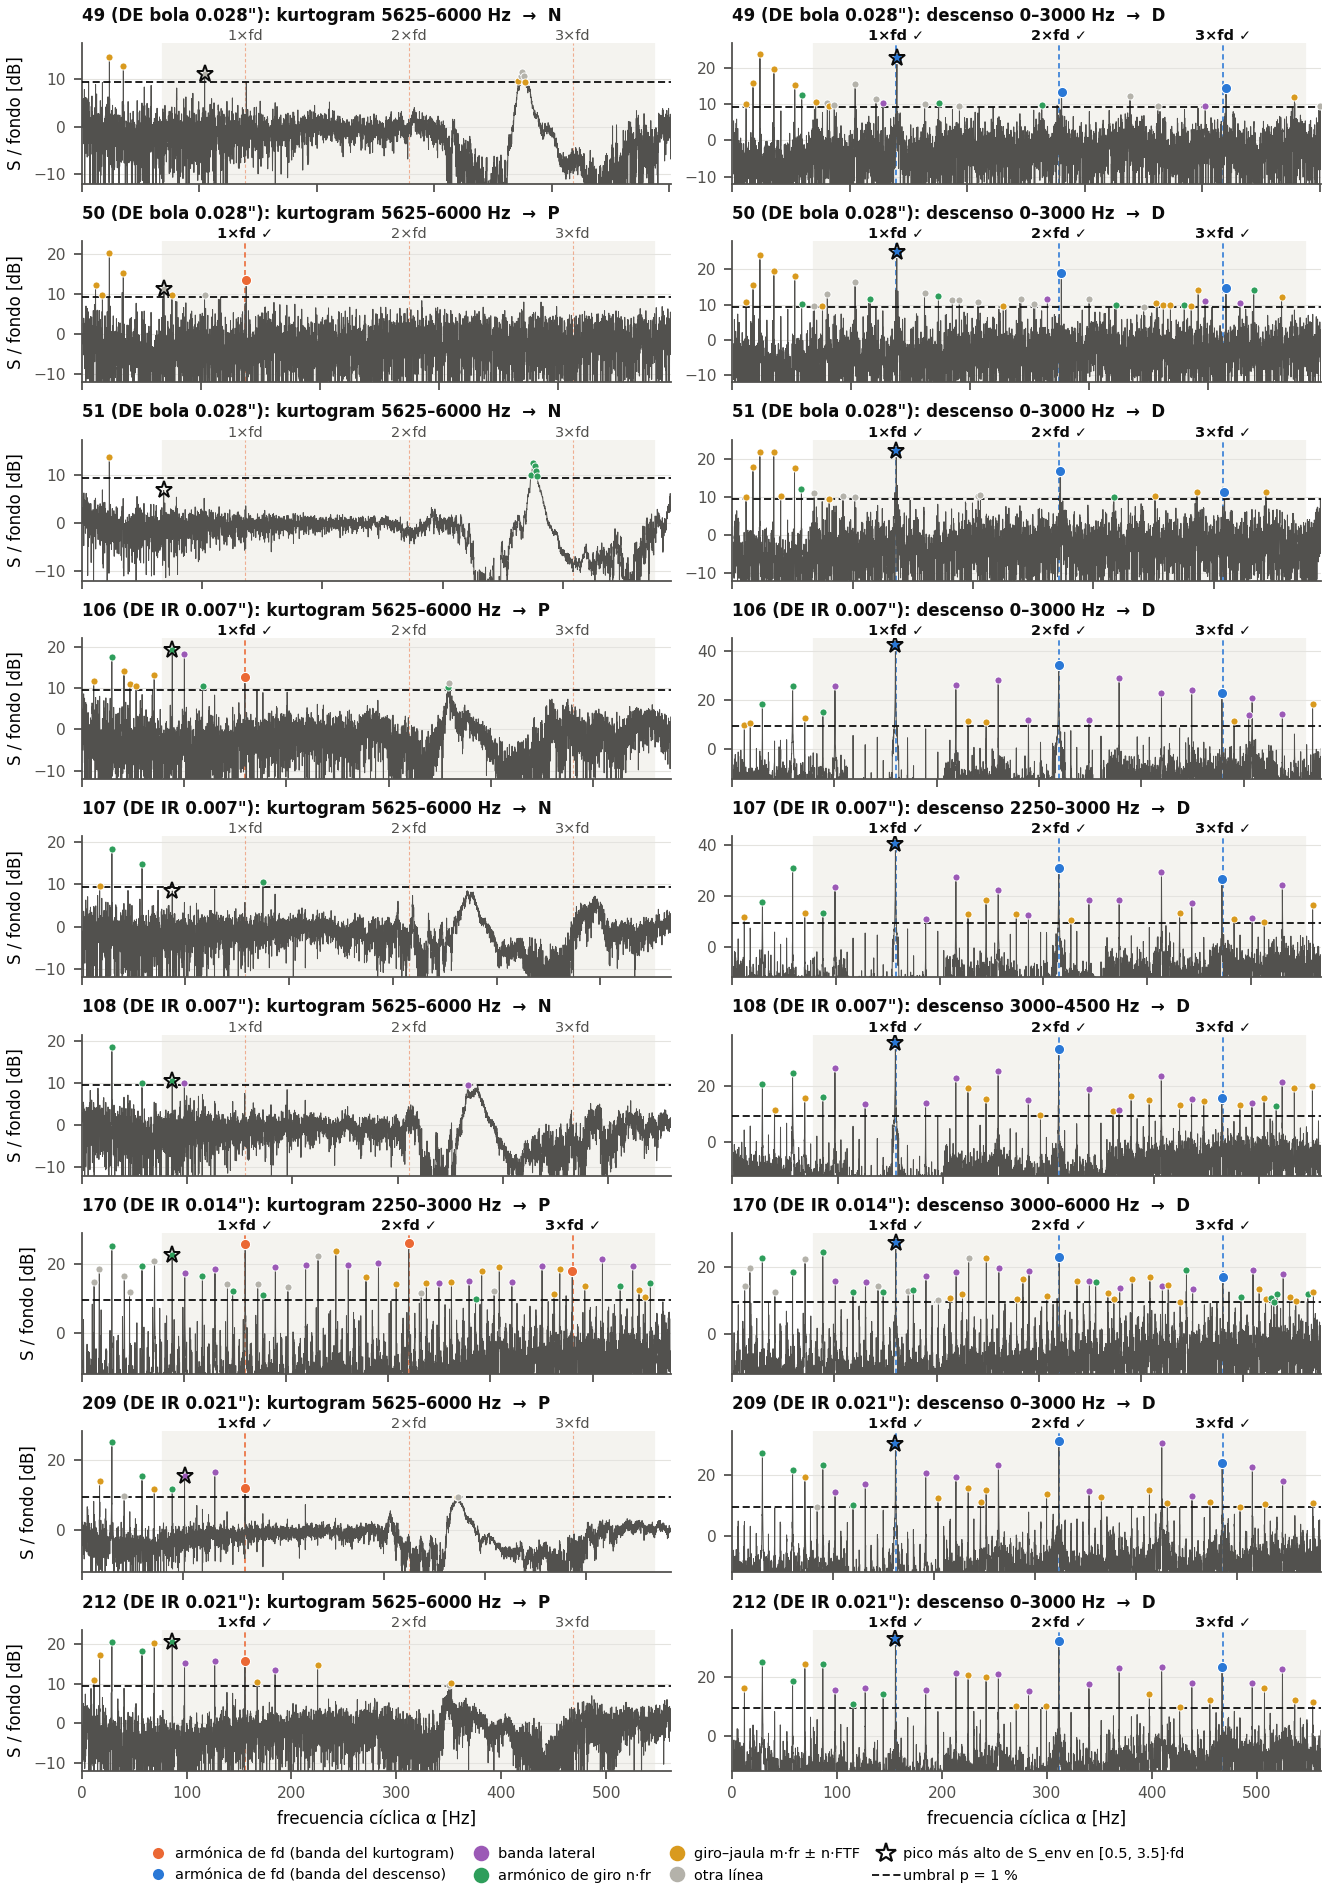
\includegraphics[width=\textwidth]{../figuras/comparacion_descenso/galeria_1.png}
\caption*{\textbf{Los 18 registros en que el descenso logra ``diagnosticable'' y el kurtogram no} (parte 1 de 2). Cada fila es un registro: a la izquierda, la envolvente relativa al fondo en la banda del kurtogram; a la derecha, la del descenso. La letra tras la flecha es el resultado (D, P o N). Mismas marcas que en las figuras anteriores.}\end{figure}
\begin{figure}[H]\centering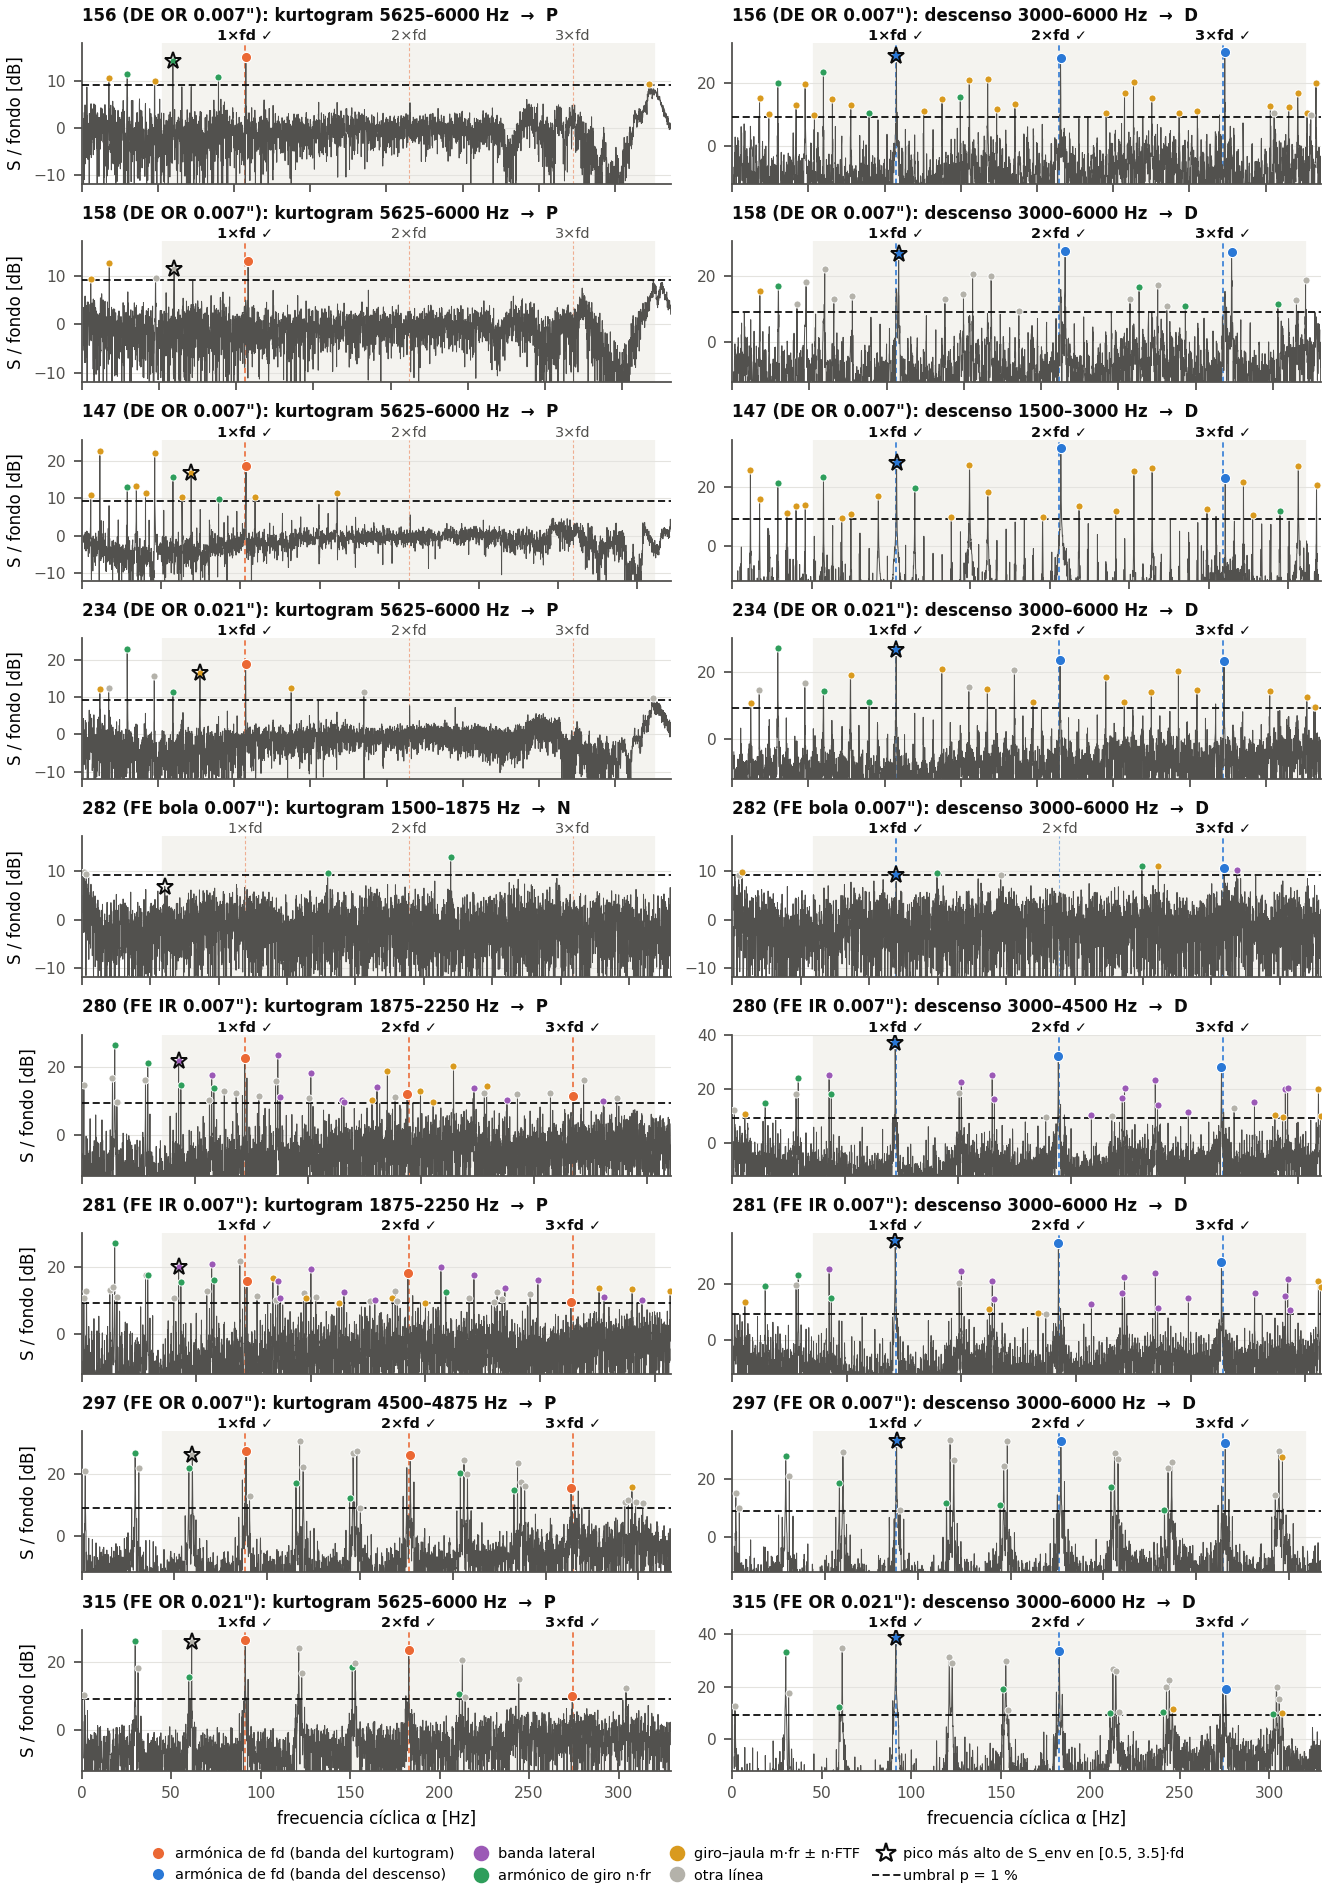
\includegraphics[width=\textwidth]{../figuras/comparacion_descenso/galeria_2.png}
\caption*{(Parte 2 de 2.) En 13 de los 18 registros el kurtogram eligió 5625--6000~Hz, junto a Nyquist. En 12 de ellos esa envolvente muestra a lo más $f_d$ entre líneas de giro y jaula; en el 315 aparecen las tres armónicas, pero domina otra línea. En los otros cinco (170, 280, 281, 297 y 282), la banda del kurtogram sí contiene las armónicas, pero otra línea domina (salvo en el 282, donde no aparece nada).}\end{figure}

\subsubsection{Casos sin ganancia y caso en contra}
\figcomp{287}{\textbf{Registro 287} (FE, bola 0{,}014~in, 1~hp; el caso parcialmente diagnosticable de la tarea). Las dos bandas son casi la misma zona (3000--4500 y 3000--6000~Hz) y dan el mismo resultado. $f_d$ es significativa por poco (10{,}9 y 10{,}7~dB, con umbral de 9{,}3~dB). $2f_d$ y $3f_d$ quedan justo bajo el umbral, y el pico más alto está en 112{,}8~Hz, un 4\% bajo $f_d$ y fuera de la ventana de $\pm2\%$: el deslizamiento de la bola ensancha y desplaza la joroba. Queda \emph{parcial} con ambos métodos.}

\figcomp{282}{\textbf{Registro 282} (FE, bola 0{,}007~in, 0~hp; el ejemplo de clase). El kurtogram elige la banda de las ráfagas no periódicas ($K=161$) y en sus ventanas no hay nada (6{,}7; 6{,}8 y 5{,}4~dB): \emph{no diagnosticable}. El descenso se detiene en 3000--6000~Hz y el criterio marca $f_d$ (9{,}3~dB, justo en el umbral de 8{,}5 veces) y $3f_d$ (10{,}6~dB); como todo es bajo, $f_d$ resulta ser el pico más alto y la regla da ``diagnosticable''. Pero el zoom muestra que el pico en $f_d$ es del mismo tamaño que otros picos del fondo. \textbf{Técnicamente D, en la práctica no diagnosticable}, como en Smith \& Randall: el descenso evita la trampa de las ráfagas, pero este registro no tiene una firma clara en ninguna banda.}

\figcomp{222}{\textbf{Registro 222} (DE, bola 0{,}021~in, 0~hp): el único registro de los 105 en que el kurtogram supera al descenso. La banda angosta del kurtogram (4875--5250~Hz) deja $f_d$ como pico dominante (13{,}3~dB): \emph{diagnosticable}. En la banda ancha del descenso (3000--6000~Hz) las tres armónicas son significativas (9{,}5; 11{,}6 y 12{,}5~dB), pero la línea más alta es una combinación giro--jaula en 161{,}9~Hz: \emph{parcial}.}

\noindent\textbf{En los 105 registros} (mismo árbol, mismo $L$, mismo criterio), el método de la tarea deja la señal \emph{diagnosticable} en 44 registros (41{,}9\%) y el descenso por sinergia en 61 (58{,}1\%). Registro por registro, el descenso gana en 18 y pierde en 1 (el 222). La tasa de ``diagnosticable'' en frecuencias señuelo es de 0--0{,}5\% para ambos, así que la mejora no viene de detectar ruido. La causa de la diferencia se ve en la galería: la curtosis premia cualquier ráfaga impulsiva, aunque no sea periódica. La sinergia, en cambio, exige que el impacto excite a la vez a los dos hijos de la banda, que es lo que hace una resonancia estructural excitada por la falla.

\section{Conclusiones}
\begin{enumerate}[itemsep=2pt]
\item Se implementaron la MFD (máscaras FFT/IFFT, curtosis compleja y kurtogram) y la envolvente espectral según las definiciones de clase. La reconstrucción de la señal por nivel es exacta a precisión de máquina.
\item \textbf{Registro 287} (FE, bola 0{,}014~in): la banda MFD 3000--4500~Hz deja ver $f_d=2\,$BSF de forma significativa, pero no dominante, junto a la modulación por la jaula (FTF). Queda \textbf{parcialmente diagnosticable}.
\item \textbf{Registro 282} (FE, bola 0{,}007~in, ejemplo de clase): la máxima curtosis ($K=161$) corresponde a ráfagas no periódicas en 1500--1875~Hz, y la envolvente filtrada no muestra $f_d$. Queda \textbf{no diagnosticable}, igual que en el benchmark de Smith \& Randall.
\item En los 105 registros, el kurtogram elige a menudo bandas dominadas por impulsos ajenos a la falla. En 19 registros la envolvente cruda era diagnosticable y la filtrada dejó de serlo. \textbf{La curtosis mide impulsividad, no periodicidad a la frecuencia de falla}: es la limitación principal del método.
\item El \textbf{descenso por sinergia}, que usa la relación padre--hijos del árbol, deja identificables las armónicas en 58\% de los registros contra 42\% del kurtogram (gana en 18 y pierde en 1), sin aumentar las falsas alarmas. El caso más claro es el registro 107, donde BPFI y sus armónicas aparecen nítidas en la banda del descenso y no aparecen en la del kurtogram.
\item \textbf{Un pico se reconoce como armónica de $f_d$} por cuatro cosas, no por su aspecto: su posición está fijada de antemano por la cinemática ($hf_d\pm2\%$); su altura se mide contra el fondo local con un umbral de falsa alarma de 1\%; para ``diagnosticable'' debe ser la línea dominante; y las armónicas deben formar una serie en múltiplos exactos (en el 107: $1:2{,}000:2{,}999$). Las demás líneas del espectro se explican casi siempre como bandas laterales $hf_d\pm kf_r$, armónicos de giro o combinaciones giro--jaula (Sección~\ref{sec:armonica}).
\item La categoría ``diagnosticable'' del criterio automático es muy específica: aparece en $\le1{,}4\%$ de frecuencias señuelo. ``Parcialmente diagnosticable'' es sensible pero poco específica, porque en CWRU la envolvente contiene muchas líneas discretas ($f_r$, FTF y sus combinaciones).
\end{enumerate}

\section*{Código entregado}
\begin{itemize}[itemsep=1pt]
\item \texttt{Fuentes.py}: MFD (máscaras, sub-señales, señal analítica, curtosis compleja, kurtogram), envolvente espectral, criterio de diagnóstico y gráficas. El núcleo usa sólo NumPy; SciPy se usa únicamente para leer los \texttt{.mat}.
\item \texttt{comparacion\_descenso.py}: figuras kurtogram vs.\ descenso por sinergia, con la envolvente relativa al fondo, los zooms por armónica y la galería de los 18 registros donde gana el descenso (Sección~\ref{sec:comp}).
\item \texttt{tarea1\_main.py}: \texttt{python tarea1\_main.py} evalúa los 105 registros; \texttt{python tarea1\_main.py 287 282} genera las figuras y fichas de esos registros.
\item Resultados en la carpeta \texttt{resultados} (tabla de todos los registros y fichas) y figuras en \texttt{figuras}, una subcarpeta por registro.
\end{itemize}


\appendix
\section{Anexo: comparación con la métrica de sinergia fraterna}
Como extensión (carpetas \texttt{02\_Sinergia\_Fraterna} y \texttt{03\_Comparacion\_Kurtogram\_vs\_Sinergia} del proyecto), se comparó el kurtogram de esta tarea con métricas que aprovechan la relación \emph{padre--hijos} del árbol MFD. La curtosis de un padre se descompone de forma exacta como $K_p=w_a^2K_a+w_b^2K_b+S_p$, donde $S_p$ (sinergia fraterna) mide la co-modulación de las envolventes de los dos hijos.

Todos los métodos se compararon con el mismo árbol, el mismo $L$ y el mismo criterio de esta tarea, sobre los 105 registros, midiendo además la tasa de ``diagnosticable'' en frecuencias señuelo.

\begin{figure}[H]\centering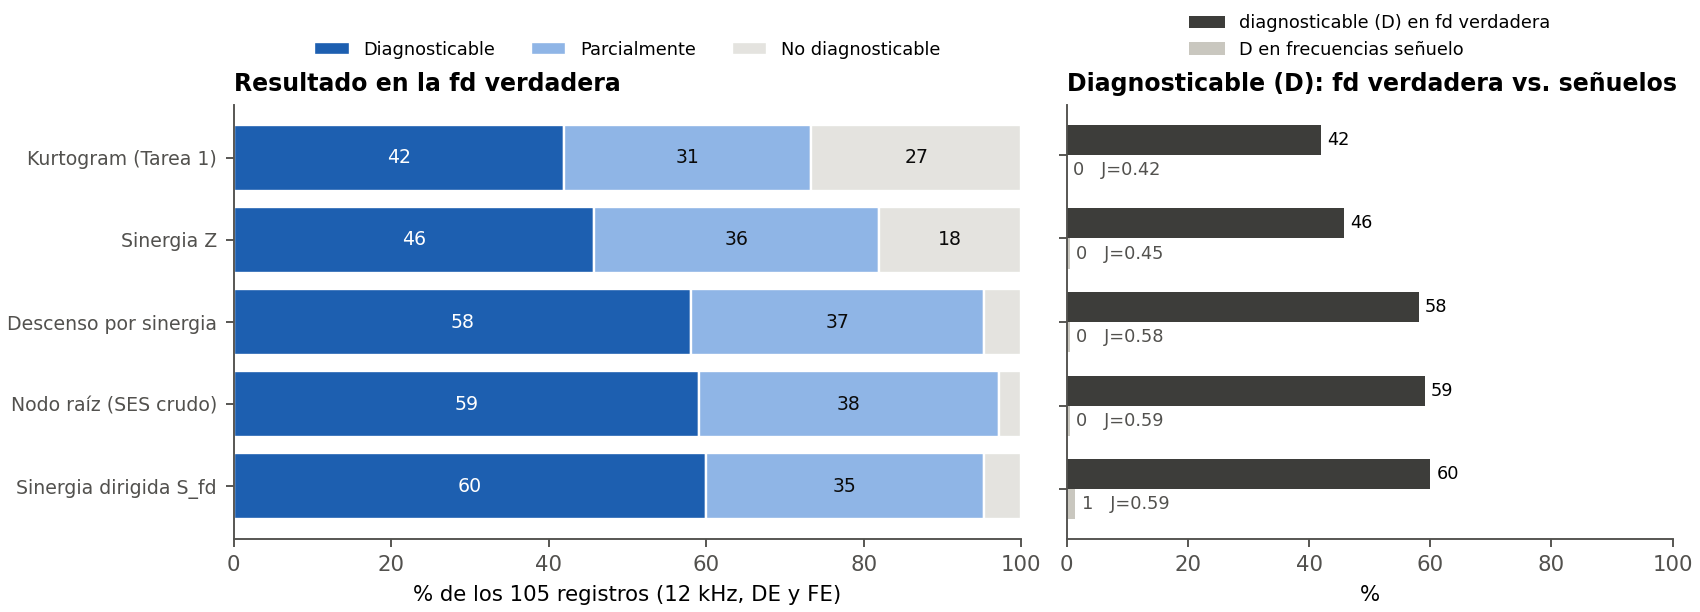
\includegraphics[width=\textwidth]{anexo_comparacion.png}
\caption*{Kurtogram de la Tarea 1 frente a métricas de sinergia (105 registros CWRU de 12~kHz). $J=$ tasa de D en $f_d$ menos tasa de D en señuelos.}\end{figure}

\begin{table}[H]\centering\small
\begin{tabular}{@{}lcccc@{}}\toprule
Método & D en $f_d$ & D en señuelos & $J_D$ & Pareado vs.\ kurtogram (gana/pierde)\\\midrule
Kurtogram (Tarea 1) & 41{,}9\% & 0{,}0\% & 0{,}42 & --\\
Sinergia $Z$ (ciega) & 45{,}7\% & 0{,}5\% & 0{,}45 & 12 / 8\\
Descenso por sinergia (ciega) & 58{,}1\% & 0{,}5\% & 0{,}58 & 18 / 1\\
Envolvente de la señal cruda & 59{,}0\% & 0{,}5\% & 0{,}59 & --\\
Sinergia dirigida $S_{f_d}$ & 60{,}0\% & 1{,}4\% & 0{,}59 & 21 / 2\\
\bottomrule\end{tabular}
\caption{Resumen de la comparación.}\end{table}

\noindent Las reglas basadas en la sinergia corrigen la principal debilidad observada del kurtogram en CWRU: elegir bandas con impulsos ajenos a la falla. El descenso por sinergia y la sinergia dirigida llegan al rendimiento de la envolvente cruda o lo superan, sin aumentar la falsa alarma.

\begin{thebibliography}{9}\small
\bibitem{sr} W.A.~Smith, R.B.~Randall, ``Rolling element bearing diagnostics using the Case Western Reserve University data: A benchmark study,'' \emph{Mech.\ Syst.\ Signal Process.} 64--65 (2015) 100--131.
\bibitem{antoni} J.~Antoni, ``Fast computation of the kurtogram for the detection of transient faults,'' \emph{Mech.\ Syst.\ Signal Process.} 21 (2007) 108--124.
\bibitem{randall} R.B.~Randall, J.~Antoni, ``Rolling element bearing diagnostics---A tutorial,'' \emph{Mech.\ Syst.\ Signal Process.} 25 (2011) 485--520.
\end{thebibliography}
\end{document}
